

\subsection{IR Based Building characteristics}
\label{sec:IRLeak}

\indent After the identifying the potentially wasteful homes, we address the problem of detecting leakages and develop more detailed heat dynamics models of the homes. We compare two different datasets - one is the individual room-wise temperature data and the other is an image sensing unit using IR camera. 

\subsubsection{\textbf{Individual Roomwise Data for Modeling Heat Dynamics:}}

\indent We have setup temperature and humidity sensors in different parts of the house and have a NEST thermostat installed. The temperatures from different parts of the house is shown in Figure~\ref{fig:Sens}. It can be seen that different parts if the house has different dynamics of temperature. This is dependent on a number of factors like exposure to sun, local heaters being used. The objective here is to get a detailed model of the house in terms of individual room-wise parameter identification considering local factors. This in turn can help us isolate the leakages or poor thermal capacity or even the  

 
 
\subsubsection{\textbf{Imaging Device}}
 

The physical component of the thermal imaging system is a custom-created imaging device as pictured in Figure~\ref{tis:imp:ex}. Our prototypes are built from a Raspberry Pi Zero, a Raspberry Pi Camera Module, and a low-resolution IR camera, powered by a $5V$ battery, rotating on a DC motor, in a 3D printed housing. This sensor's purpose is to collect data from which to create a longitudinal thermal
map of a room and from which to detect the variations representing leakages and other energy waste.

There are two cameras in the imaging device. The IR camera is Melexis MLX90621~\cite{MLX}, which is a low resolution ($16\times$) and low power consumption of $<9mA$ when active and $<7\mu A$ otherwise. It can detect ambient temperature between  -40$^{\circ}$C  and 85 $^{\circ}$C  and object temperatures between  -50$^{\circ}$C  and  300$^{\circ}$C  with a resolution of  0.02$^{\circ}$C. The Raspberry Pi Camera Module~\cite{picam} is a RGB camera and collects images at $720\times480$ resolution. The 3D printed housing holds the cameras in a consistent relative position and orientation. The Raspberry Pi Zero controls the device and rotates the sensor unit (at 15min-1hour interval as per setting) for a number of steps sufficient to rotate at
least  360$^{\circ}$C. For every step, the Pi collects a simultaneous image from each camera. After the batch of rotations completes, the imaging device uploads the collected images to a server for processing.



%\textsc{\begin{figure}[t!]
%\begin{center}
%	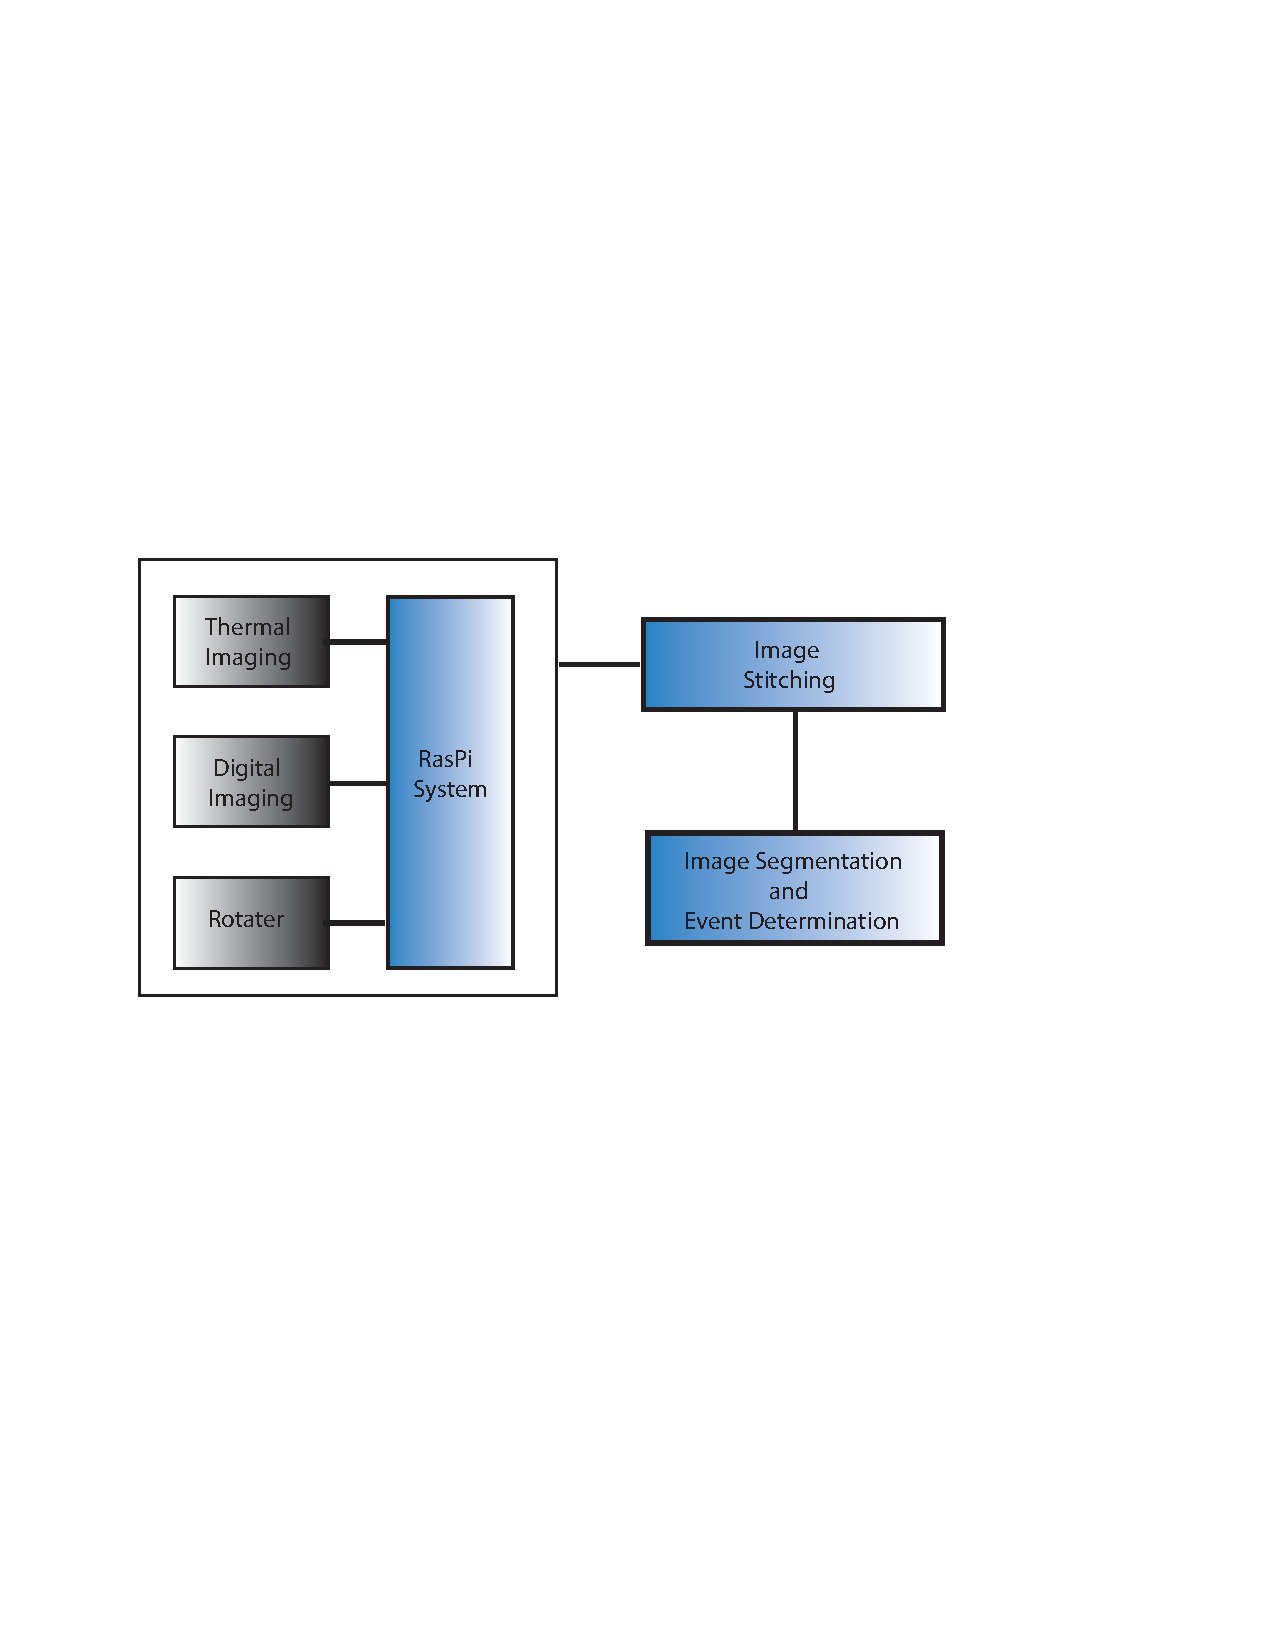
\includegraphics[width=3.5in]{figs/SystemArch.pdf}
%\end{center}
%  \caption{Thermal Imaging System Block Diagram}
%  \label{fig:Overview}
%\end{figure}}

	
\begin{figure}[h]
 \centering
    \subfloat[Imaging Device]{
      \label{tis:imp:ex}
        %\subcaption{House 2470: $T_a$,$T_i$ \& $\dc$}
        \includegraphics[height=.2\textheight,width=.15\textwidth,keepaspectratio]{CameraModule.jpg}
    }
       \centering
    \subfloat[Room-wise Temperature Sensor Data]{
      \label{fig:Sens}
        %\subcaption{House 2470: $T_a$,$T_i$ \& $\dc$}
        \includegraphics[height=6cm,width=.35\textwidth,keepaspectratio]{Temp.jpeg}
    }
    \caption{Imaging Device and Room-wise Temperature Data}
\end{figure}

\subsubsection{\textbf{Image Processing}}
 \indent On the image processing server, we use the RGB and IR image sets to generate a unified thermal map of the room. The first image processing step uses OpenCV to generate a panorama from the RGB images and record the homography matrices used for those image transformations. This process allows us to avoid the need for a heavier, more expensive stepper motor, because those homography matrices encode the relationships between sequential images. The second step uses those  matrices to produce an IR panorama of the room. The 3D printed housing of the imaging device maintains a fixed relationship between the positions and perspectives of the two cameras in each prototype. We calculate the mapping between the cameras once and, at processing time, use this transformation in addition to the homographies calculated in the RGB stitching process. Thus, we map each IR image on to its corresponding RGB image, then stitch those transformed IR images to create an IR panorama of the room.

\indent We propose to use the IR camera in tandem with a digital camera to detect and appropriately map the heatmap's points of interest in contrast to the presence of buildings air leakages, heat dissipation associated with different objects and appliances while achieving high precision and detection accuracy. While the specific color codes of heatmaps help detect the moderate, extreme or regular hot and cold surfaces, augmenting this with digital images helps detect any unusual usage behaviors, and operating conditions of everyday appliances in a smart home environment. For example, if a room has multiple windows and doors with air leakages or multiple similar small to medium load appliances, solely the heatmaps may not provide the home owners the adequate information as needed to detect any abnormal energy usage. While the IR camera albeit helps detect the region of interest but fails to provide the detailed identifications of the similar type of objects and appliances.

 
\indent We employ the digital stitching procedure~\cite{Stitch} to create the thermal panorama. We first stitch the digital images and maintain the respective control points for the stitching procedure which we reemploy to process the stitched thermal image generation. Next we augment the digital image in the background of the stitched thermal image based on the respective control points. We use a hybrid image construction methodology where the mask image or the thermal image is passed through a low pass filter and the digital image is passed through a high frequency filter to construct the digital image augmented heatmaps. We then apply a image segmentation algorithm to determine the different heatzone clusters in the stitched image. The temperature of each cluster is them compared with entries in a lookup table to determine the state of a specific appliance.  
 
\subsubsection{\textbf{Initial Image Analytics}}

There are three possible types of thermal regions in an image - background, cold region and hot region. The image that needs to be segmented is the stitched IR image and the objective is to create a thermal mask which separates the hot and cold regions from the background. Since the thermal image is being used for segmentation, the results are subject to the choice of color palette and range selection.  We ensure that the background has darker tones than the hot or cold surfaces which helps achieve the desired segmentation after image binarization using Otsu's method~\cite{OTSU}. We apply a 7$\times$7 neighborhood 2-D median filter to eliminate small blobs and isolate the few major thermal zones. Initial experiment suggested that the it is easy to detect human presence and objects as long as the wall temperature do not mask them. In Figure~\ref{fig:IR}, shows two sample stitched images during different time duration. It can be seen that there is a slight cool area detected near the window given in a deeper shade of blue. 

\begin{figure}[t]
 \centering
    \subfloat[Sample 1]{
      \label{fig:IR1}
        %\subcaption{House 2470: $T_a$,$T_i$ \& $\dc$}
        \includegraphics[height= 2cm,width=4cm]{overlay1}
    }
       \centering
    \subfloat[Sample 2]{
      \label{fig:IR2}
        %\subcaption{House 2470: $T_a$,$T_i$ \& $\dc$}
        \includegraphics[height=2cm,width=4cm]{overlay2}
    }
    \caption{Overlapped Room Image and IR image}
    \label{fig:IR}
\end{figure}

\indent The challenges in stitching mainly stem from our simple approach. Better image stitching can solve the problem. Alternatively, rotating the unit on a stepper motor, instead of DC motor, can be another solution which can up the unit price by \$8. We're doing feature-detection based stitching, which has a lot more difficulty with close-up objects and with blank, featureless walls and the unit positioning is another factor. Ideally keeping the unit centered in the room may solve the problem however that can cause logistical problems.  